%mscS --> seminar
%msc --> Thesis

% برای گزارش سمینار mscS  و برای پایان‌نامه ,msc را انتخاب کنید
\documentclass[oneside,openany,mscS]{SBU-Thesis}
\usepackage{graphicx}
\usepackage{subcaption}
\usepackage{verbatim}
\usepackage{booktabs}
\usepackage[thinlines]{easytable}
\usepackage{adjustbox}
\usepackage[graphicx]{realboxes}
% برای وارد کردن بسته‌هایی که نیاز است قبل از bidi وارد شوند، آنها را در فایل confix.tex قرار دهید. سایر بسته‌های مورد نیاز را در اینجا می‌توانید وارد کنید:

\begin{document}
	%عنوان پایان‌نامه
	\title{بررسی و ارزیابی راهکارهای رندرینگ در واقعیت افزوده}
	
	%رشته
	\subject{مهندسی کامپیوتر}
	
	%گرایش
	\field{نرم‌افزار}
	
	%نام
	\name{محسن}
	
	%نام خانوادگی
	\surname{نوازنی}
	
	%استاد راهنما
	\firstsupervisor{دکتر مجتبی وحیدی اصل}
	
	%استاد راهنمای دوم (در صورت وجود، در غیر این صورت این خط را حذف کنید)
%	\secondsupervisor{دکتر محمود نشاطی}

	%استاد مشاور (در صورت وجود، در غیر این صورت این خط را حذف کنید)
%	\firstadvisor{دکتر محمود نشاطی}

%تاریخ انجام پایان‌نامه
	\thesisdate{تابستان ۱۳۹8}
	
	%نام دانشکده
	\faculty{دانشکده مهندسی و علوم کامپیوتر}
	
	%نام دانشگاه
	\university{دانشگاه شهید بهشتی}
	
	%اسامی برای صفحات داوران: در هر مورد، در صورت عدم وجود، کل خط را حذف کنید
	\davaranSupervisor{نام و نام‌خانوادگی}
	\davaranSecondSupervisor{نام و نام‌خانوادگی}
	\davaranAdvisor{نام و نام‌خانوادگی}
	\davaranInternal{نام و نام‌خانوادگی}
	\davaranExternal{نام و نام‌خانوادگی}
	\davaranAssignee{نام و نام‌خانوادگی}
%	\davaranDate{۱۳۹۷/۱۱/۷} % چنانچه این خط را حذف کنید با فضای خالی جایگزین می‌شود

	%مقادیر انگلیسی برای صفحه آخر
	\latinuniversity{Shahid Beheshti University}
	\latinfaculty{Faculty of Computer Science \& Engineering}
	\latintitle{Review and evaluate rendering strategies in Augmented Reality}
	\latinname{Mohsen}
	\latinsurname{Navazani}
	\latinthesisdate{2019}
	\firstlatinsupervisor{Dr. Mojtaba Vahidi Asl}
	%	\secondlatinsupervisor{Dr. Mahmood Neshati}
	%	\firstlatinadvisor{Dr. Mahmood Neshati}
	% چکیده به فارسی
	\fa-abstract{واقعیت افزوده فنّاوری است که با مخلوط کردن واقعیت و مجازی، توجه زیادی از جامعه علمی را به خود جلب کرده است و بهترین راه برای انتقال اطلاعات مربوط به دنیای واقعی به افراد است. رایانه‌ها گرافیک‌هایی را تولید کرده و بر روی دنیای واقعی ثبت می‌کنند و به این شکل به نظر می‌رسد که این گرافیک‌ها به دنیای  واقعی افزوده‌شده‌اند، برای همین به این فنّاوری واقعیت افزوده گفته می‌شود.
		ما شاهد رشد فنّاوری‌های جدید مانند هوش مصنوعی و همچنین گستردگی محصولات موجود در بازار فنّاوری هستیم، باوجود گذشتن چند دهه از به وجود آمدن واقعیت افزوده، این فنّاوری طرفداران زیادی چه در حوزه اقتصادی و چه در حوزه علمی به خود اختصاص داده است.
		مطالعات زیادی بر روی این فنّاوری انجام‌شده است ولی بااین‌وجود، دارای مسائل حل‌نشده و جای کار بسیاری است. درنتیجه می‌تواند حوزه خوبی برای تحقیق برای علاقه‌مندان باشد.
		در این تحقیق سعی بر آن بوده است که در اول انگیزه از این پژوهش و دلایل انتخاب این موضوع آورده شود، سپس به معرفی سیستم واقعیت افزوده پرداخته و اجزا این سیستم و روش کار هرکدام به‌اختصار توضیح داده شود  و در آخر مسئله رندرینگ شرح داده‌شده و در آن تمرکز بر روی مسئله ردیابی بوده است و درنهایت انواع روش‌های آن شرح داده می‌شود و با یکدیگر مقایسه می‌شوند.}
	%کلمات کلیدی:
	\keywords{واقعیت افزوده، رندرینگ، ردیابی}
	%%%%%%%%%%%%%%%%%%%%%%%%%%%%%%%%%
	
	
\firstPage %ساخت صفحه اول پایان‌نامه 
\davaranPage % ساخت صفحه امضا داوران

%%%%%%ساخت صفحه تقدیر و تشکر%%%%%%%%%%
{
	\newpage
	\thispagestyle{plain}
	\noindent
	\large{\textbf{با سپاس و قدردانی از}}
	
	\noindent
	پدران و مادرانی که خود را فدای تربیت فرزاندان خود کردند و\\
	اساتید و معلمانی که در تمام دوران زندگی، راهنمای جانسوز ما بودند.
	
	
	\vspace{14cm}	
	
	
	\pagebreak
}
%%%%%%%%%%%%%%%%%%%%%%%%%%%%%%%%

\rightsPage % ساخت صفحه حقوق پایان‌نامه
\copyRightPage % ساخت صفحه تعهدنامه

%%%%%%ساخت صفحه تقدیم به %%%%%%%%%%
{
	\newpage
	\thispagestyle{plain}
	\large{\textbf{تقدیم به}}
	
	\begin{center}
		رهجويان علم و فناوری و دوست‌داران علم و دانش
	\end{center}
	
	\vspace{14cm}	
	
	
	\pagebreak
}
%%%%%%%%%%%%%%%%%%%5
\tableofcontents % فهرست مطالب
\listoffigures \newpage % فهرست تصاویر
\listoftables \newpage % فهرست جداول

	
\abstractPage % ساخت صفحه چکیده
		

%%%%%%%%%%%%%%%%%%%%%%%%%%%

\cchapter{مقدمه}
\section{واقعیت افزوده چیست؟}
در سال ۱۹۷۷ خیلی از علاقه‌مندان به فیلم و سینما، با دیدن تصویر ۳ بعدی از زنی در هوا که در حال گفتن جمله‌ی،  \lr{"Help me Obiwan-Kenobi you’re my only hope"} بود، شگفت‌زده شدند. این صحنه فوق‌العاده متعلق به فیلم \lr{Star Wars} \LTRfootnote{http://www.starwars.com}بود که با استفاده از افکت‌های مخصوص توانسته بودند محتوای ۳ بعدی و مجازی را در دنیای واقعی خلق بکنند. این فیلم صحنه‌ای از آینده را نشان می‌داد که در آن مردم می‌توانستند در دنیایی که اجسام واقعی و مجازی باهم ترکیب‌شده‌اند، به‌راحتی مانند دنیای واقعی با کامپیوترها ارتباط برقرار بکنند.
\\
حدود ۳۰ سال بعد در سال ۲۰۰۸، در میان برگزاری انتخابات ریاست جمهوری آمریکا، یک نمایشِ ویژه از تکنولوژی به مردم نشان داده شد. در میان صحبت در رابطه با انتخابات توسط شبکه \lr{CNN}، خبرنگار \lr{Wolf Blitzer }به سمت جایگاه خالی نگاه کرد و ناگهان خبرنگار \lr{Jessica Yellin } بر روی صحنه به‌صورت ۳ بعدی و درون برنامه زنده ظاهر شد\LTRfootnote{http://edition.cnn.com/2008/TECH/11/06/hologram.yellin/}. \lr{Wolf} قادر بود با او، صحبت کند و یک مکالمه زنده و رودررو داشته باشد درصورتی‌که \lr{Jessica Yellin }  هزاران مایل با او فاصله داشت.
\\
این‌یک مثال از واقعیت افزوده بود \LTRfootnote{Augmented Reality} که به‌اختصار به آن \lr{AR} نیز گفته می‌شود که قادر است تصاویر مجازی را بسازد و به دنیای واقعی اضافه کند. واقعیت افزوده تکنولوژی است که در دسته فنّاوری‌های مرتبط با ارتباط انسان و کامپیوتر \LTRfootnote{human computer interaction technology} قرار می‌گیرد، که در این دسته فنّاوری‌هایی قرار می‌گیرند که باعث برقراری ارتباط  بهتر انسان و کامپیوتر می‌گردند و شروع این تکنولوژی‌ها از حدود دهه ۱۹۶۰ است با به وجود آمدن کارت‌های پانچ شروع شد و در ادامه این روند به موس‌ها، کیبوردها و ... رسید. هدف این تکنولوژی این است که رابط کاربری  کاربران که درک و ارتباط با آن دشوار است را از دید آن‌ها مخفی کند و ارتباط با کامپیوتر را بسیار ساده‌تر مانند ارتباط با دنیای واقعی بکند.
\\
مثال‌های بالا به ما نشان می‌دهد که واقعیت افزوده چقدر در ارتباطات و نمایش اطلاعات می‌تواند به ما کمک بکند و همین‌طور مانند تکنولوژی‌های دیگر، واقعیت افزوده می‌تواند در سطح خیلی گسترده‌تری نیز به‌کار برود. محققین تا به امروز در حوزه‌های مختلفی از این تکنولوژی استفاده کرده‌اند مانند پزشکی، سرگرمی، مهندسی، آموزش نظامی و غیره. برای نمونه در پزشکی می‌توان اطلاعات بیمار را بر روی بدن فرد بیمار به نمایش درآورد \cite{nasir}و در رابطه با سرگرمی، بازیکنان می‌توانند در دنیای واقعی به بازی بپردازند \cite{Piekarski}و یا در مهندسی، مهندسان می‌توانند انتهای یک پروژه ساختمانی را ببینند\cite{Fjeld}.
\\


	\begin{figure}
		\centering
		\begin{subfigure}[b]{0.4\textwidth}
			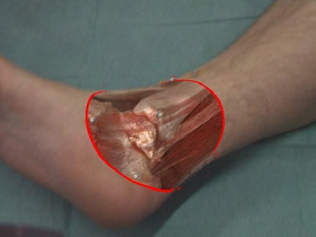
\includegraphics[width=\textwidth]{image/AR_in_medicine}
			\caption{استفاده از واقعیت افزوده در پزشکی
			\\
		\cite{nasir}}
			\label{fig:gull}
		\end{subfigure}
		~ %add desired spacing between images, e. g. ~, \quad, \qquad, \hfill etc. 
		%(or a blank line to force the subfigure onto a new line)
		\begin{subfigure}[b]{0.4\textwidth}
			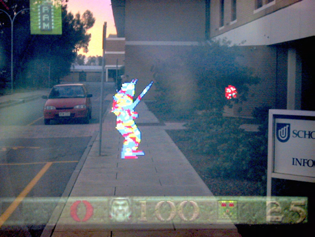
\includegraphics[width=\textwidth]{image/ARQuake_outdoor_AR_game}
			\caption{استفاده از واقعیت افزوده برای بازی
			\\
			\cite{Piekarski}}
			\label{fig:tiger}
		\end{subfigure}
		~ %add desired spacing between images, e. g. ~, \quad, \qquad, \hfill etc. 
		%(or a blank line to force the subfigure onto a new line)
		
		\begin{subfigure}[b]{0.4\textwidth}
			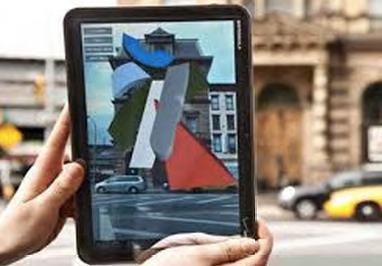
\includegraphics[width=\textwidth]{image/AR_architecture_by_Re+Public}
			\caption{استفاده از واقعیت افزوده در مهندسی
			\\
			\cite{Fjeld}}
			\label{fig:mouse}
		\end{subfigure}
		\caption{انواع استفاده از واقعیت افزوده}\label{fig:َARType}
	\end{figure}

\section{تاریخچه}
گرچه واقعیت افزوده امروزه محبوب شده است، اما این فنّاوری جدید نیست، برای هزاران سال مردم از آینه‌ها، منابع نوری و ... برای ایجاد تصاویر مختلف در دنیای واقعی استفاده می‌کردند. برای مثال در قرن ۱۷ ام تئاترها و موزه‌ها از آینه‌های متعددی  برای ادغام انعکاس اجسام و افزودن تصویری مجازی به دنیای واقعی استفاده می‌کردند\cite{Brooker}. \lr{Ivan Sutherland} اولین کسی بود که با استفاده از رایانه‌ها در دانشگاه ام آی تی \LTRfootnote{Massachusetts Institute of Technology} و در سال ۱۹۶۳ توانست تصاویر مجازی را به دنیای واقعی بیاورد\cite{Sutherland}. او در سال ۱۹۶۸ به دانشگاه هاروارد \LTRfootnote{Harvard University} رفت و در آنجا با کمک \lr{Bob Sproull } توانستند اولین دستگاه واقعیت افزوده را بسازند\cite{Sutherland2}. این دستگاه بر روی سر قرار می‌گرفت و با استفاده از تابش نور بر روی عدسی‌ای مقابل چشمان سعی بر آن داشت تا تصاویر مفهومی را به بیننده نمایش دهد. برای ایجاد تصاویر ۳ بعدی از چندین عدسی و با استفاده از تابش‌های مختلف در جهات مختلف، توانستند تصاویر ۳ بعدی را بسازند\cite{Sutherland2}.
\\
\begin{figure}
	\centering
	\begin{subfigure}[b]{0.3\textwidth}
		\includegraphics[width=\textwidth]{image/Sutherland’s2}
		
		\label{fig:gull}
	\end{subfigure}
	~ %add desired spacing between images, e. g. ~, \quad, \qquad, \hfill etc. 
	%(or a blank line to force the subfigure onto a new line)
	\begin{subfigure}[b]{0.6\textwidth}
		\includegraphics[width=\textwidth]{image/Sutherland’s1}
		
		\label{fig:tiger}
	\end{subfigure}
	~ %add desired spacing between images, e. g. ~, \quad, \qquad, \hfill etc. 
	%(or a blank line to force the subfigure onto a new line)
	
	\caption{سیستم واقعیت افزوده طراحی شده توسط Sutherland ، ۱۹۶۸ \cite{Sutherland2}}\label{fig:Sutherland1968}
\end{figure}

در سال‌های بعد، تحقیق بر روی این فنّاوری علاوه بر دانشگاه‌ها، در آزمایشگاه‌های نظامی و دولتی نیز شروع شد و موردتوجه قرار گرفت. به‌عنوان‌مثال \lr{Tom Furness} در آزمایشگاه‌های هوا و قضای آمریکا، بر روی این فنّاوری شروع به تحقیق نمود و پروژه ای بانام \lr{Super-Cockpit} را شروع کرد که به آموزش خلبانان هواپیما کمک می‌کرد\cite{Furness}.
\begin{figure}
	\centering
	\begin{subfigure}[b]{0.4\textwidth}
		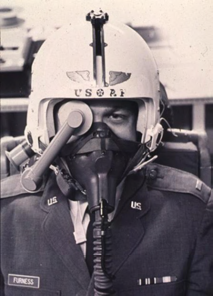
\includegraphics[width=\textwidth]{image/airforce1}
		\caption{دوربین نصب شده بر روی سر یک خلبان}
		\label{fig:gull}
	\end{subfigure}
	~ %add desired spacing between images, e. g. ~, \quad, \qquad, \hfill etc. 
	%(or a blank line to force the subfigure onto a new line)
	\begin{subfigure}[b]{0.5\textwidth}
		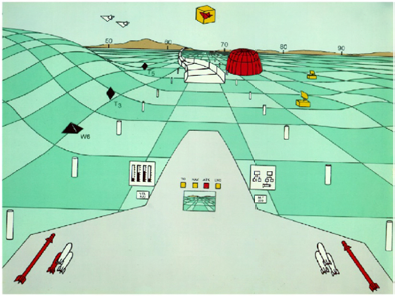
\includegraphics[width=\textwidth]{image/airforce2}
		\caption{تصویر شبیه سازی شده در پروژه}
		\label{fig:tiger}
	\end{subfigure}
	~ %add desired spacing between images, e. g. ~, \quad, \qquad, \hfill etc. 
	%(or a blank line to force the subfigure onto a new line)
	
	\caption{پروژه Super-Cockpit \cite{Furness2}}\label{fig:Super-Cockpit}
\end{figure}


در سال ۱۹۸۱ آژانس ملی فضا و هواشناسی \lr{(NASA)} شروع به تحقیق بر روی این فنّاوری نمود و کلاه و نمایشگر مخصوص به خود را نیز طراحی کرد که می‌توانست برای آموزش فضانوردان با ایجاد تصاویر مجازی کمک بکند\cite{Furness2}.
\\
\section{انگیزه پژوهش}
\noindent
گارتنر\LTRfootnote{Gartner}، شرکت پژوهشی و مشاوره آمریکایی است، که درزمینه ارائه خدمات برون‌سپاری، تحقیق و پژوهش و مشاوره فناوری اطلاعات فعالیت می‌نماید. شرکت گارتنر در سال ۱۹۷۹ توسط Gideon Gartner راه‌اندازی شد و در حال حاضر دارای عملیات در ۸۵ کشور جهان است. دفتر مرکزی این شرکت در شهر استنفورد، کنتیکت، ایالات‌متحده آمریکا قرار دارد و سهام آن در بازار بورس نیویورک معامله می‌شود\LTRfootnote{https://en.wikipedia.org/wiki/Gartner}.
\\
این شرکت هرساله نموداری را معرفی می‌کند که در آن به معرفی تکنولوژی‌های روز پرداخته و موقعیت آنها آن‌ها را بررسی می‌کند\LTRfootnote{https://www.gartner.com/smarterwithgartner/5-trends-emerge-in-gartner-hype-cycle-for-emerging-technologies-2018/}.شکل:\ref{fig:gartner}
\\

\begin{figure}[tb]
	\centering
	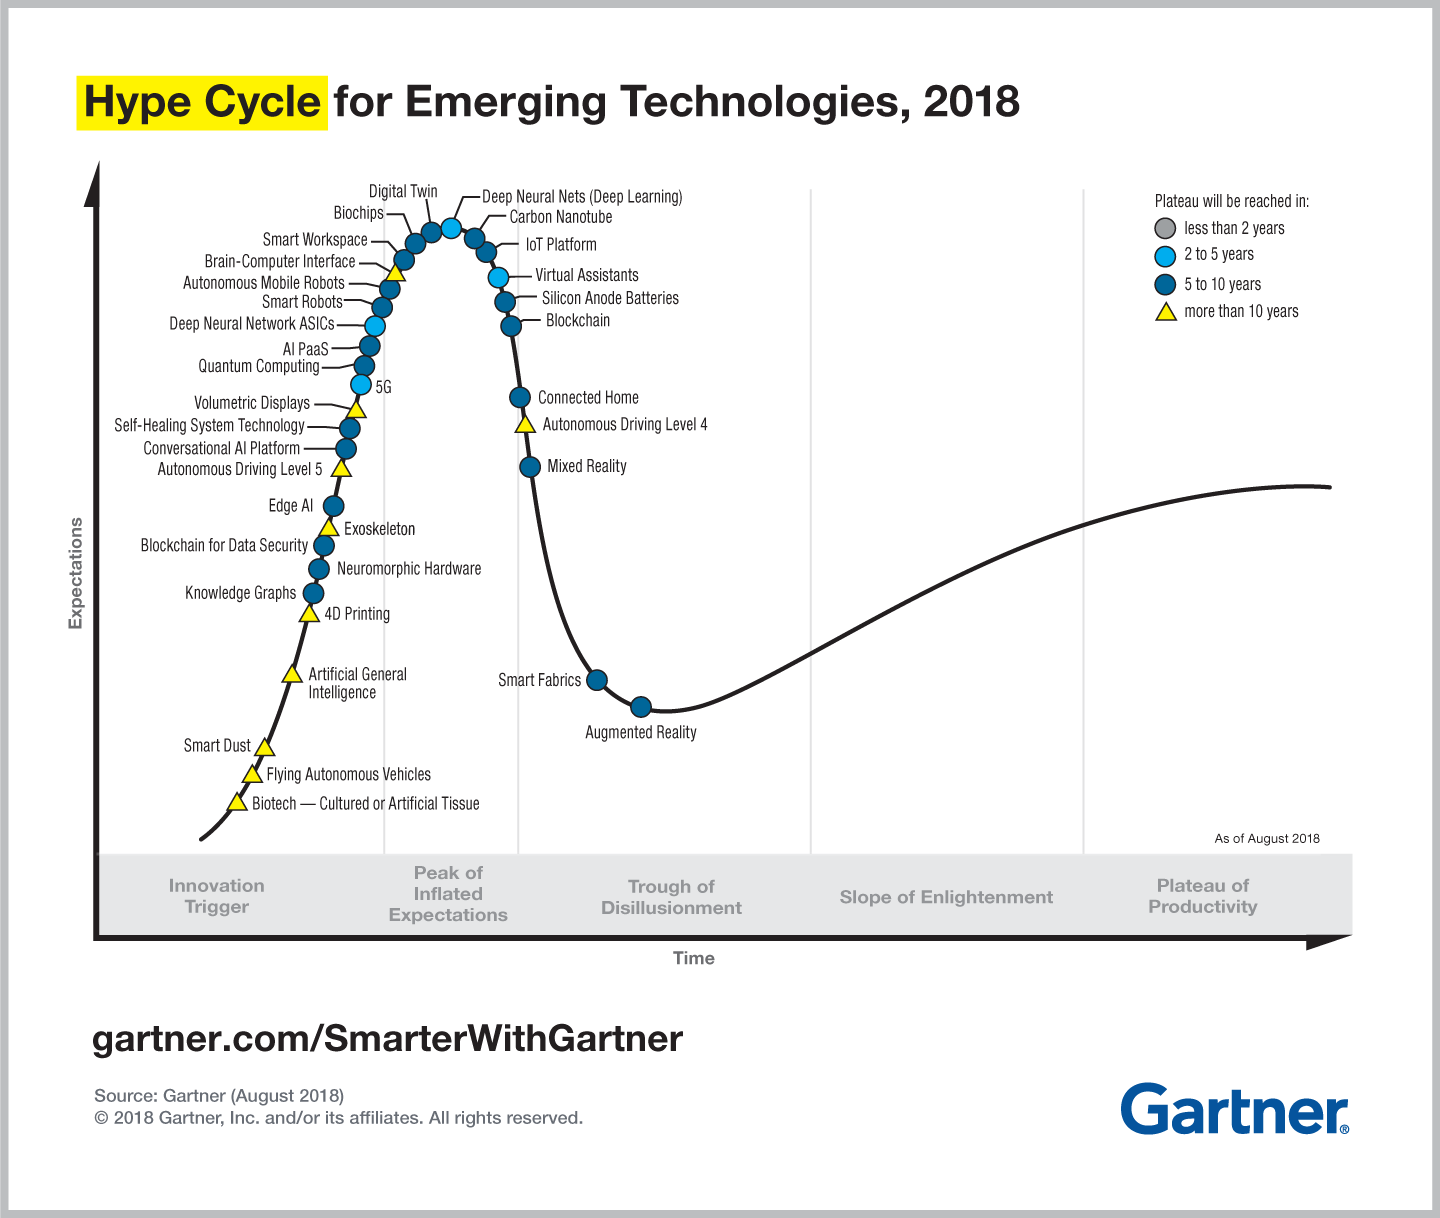
\includegraphics[width=1\linewidth]{image/gartner}
	\caption {نمودار موقعیت فنّاوری‌ها در سال ۲۰۱۸}
	\label{fig:gartner}
\end{figure}
\noindent
این نمودار از ۵ قسمت مختلف تشکیل‌شده است: 
\\
\textbf{
	۱-راه افتادن فنّاوری \LTRfootnote{Technology Trigger} : }در این مرحله یک فنّاوری مفهوم‌سازی می‌شود، پتانسیل‌های آن موردبررسی قرار می‌گیرد و شروع به اثبات ادعاهای خود می‌کند.
\\
\textbf{
	۲-اوج انتظارات \LTRfootnote{Peak of Inflated Expectations} : }در این مرحله تکنولوژی به پیاده‌سازی می‌رسد و نظریات و تبلیغات در رابطه با موفقیت‌آمیز بودن و یا نبودن آن مطرح می‌شود.
\\
\textbf{
	۳-مرحله سرخوردگی \LTRfootnote{Trough of Disillusionment} :} در این مرحله مشکلات تکنولوژی نمایان می‌شود و شروع تلاش‌ها برای رفع این مشکلات است.
\\
\textbf{
	۴-شیب روشنگری \LTRfootnote{Slope of Enlightenment} :} در این مرحله شرکت‌های مختلف به این تکنولوژی روی می‌آورند و پتانسیل‌های این فنّاوری برای آینده نمایان‌تر می‌شود.
\\
\textbf{
	۵-فلات بهره‌وری \LTRfootnote{Plateau of Productivity} :} در اینجا استفاده از این فناوری گسترده و همه‌گیر شده و تعداد خیلی زیادی از شرکت‌های کوچک و بزرگ به آن روی می‌آورند.
\\
همان‌طور که ملاحظه می‌شود این فنّاوری در مرحله سوم قرار دارد و مشکلاتی دارد که باعث می‌شود زمینه خوبی برای مطالعه و تحقیق باشد و همچنین بسیار گرایش برای آن وجود دارد به‌طوری‌که شرکت بزرگی مانند Gartner این فنّاوری را پیشنهاد می‌دهد و پیش‌بینی می‌کند که یکی از فنّاوری‌هایی باشد که در آینده نزدیک شاهد ظهور و گسترده شدن آن خواهیم بود.
\\
یکی از مراجع مهم و معروف برای مقاله‌ها در این زمینه، نشست بین‌المللی واقعیت افزوده و واقعیت ترکیبی \lr{(ISMAR)}\LTRfootnote{International Symposium on Mixed and Augmented Reality (ISMAR)} است که در قالب \lr{IEEE Computer Society } به‌صورت سالیانه برگزار می‌شود، با بررسی و ارزیابی ۲ دهه از مقاله‌های منتشرشده در این کنفرانس، به نمودارهای زیر می‌رسیم.‌\RTLfootnote{در این مقاله منظور از \lr{Rendering} نحوه پردازش تصویر است و با واژه رندرینگ در این تحقیق متفاوت است. }\cite{ismar}.
\begin{figure}
	\centering
	\begin{subfigure}[b]{1\textwidth}
		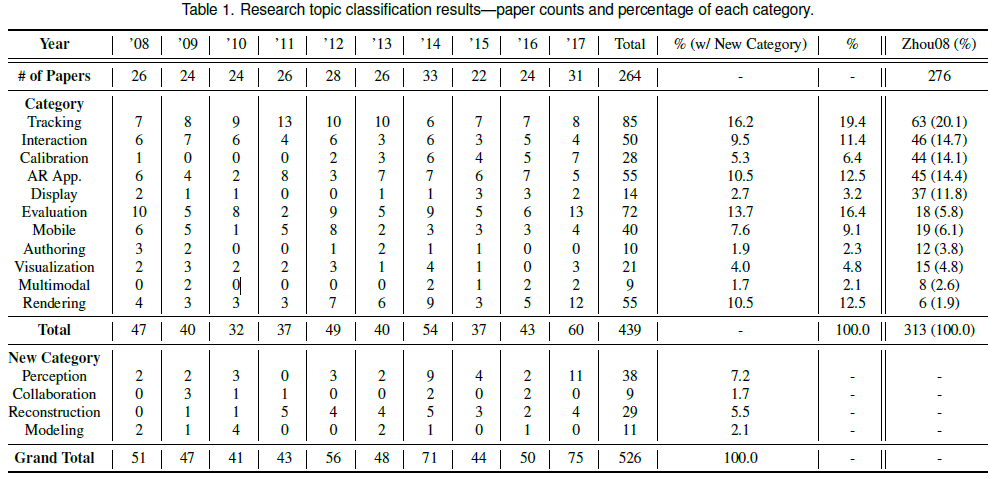
\includegraphics[width=\textwidth]{image/ismar1}
		\caption{تعداد مقاله ها بر اساس موضوع}
		\label{fig:gull}
	\end{subfigure}
	~ %add desired spacing between images, e. g. ~, \quad, \qquad, \hfill etc. 
	%(or a blank line to force the subfigure onto a new line)
	\begin{subfigure}[b]{0.4\textwidth}
		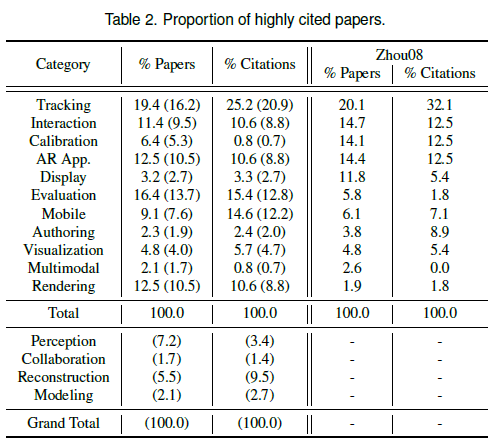
\includegraphics[width=\textwidth]{image/ismar2}
		\caption{ارجاع به مقالات به نسبت تعداد}
		\label{fig:tiger}
	\end{subfigure}
	~ %add desired spacing between images, e. g. ~, \quad, \qquad, \hfill etc. 
	%(or a blank line to force the subfigure onto a new line)
	\begin{subfigure}[b]{0.5\textwidth}
		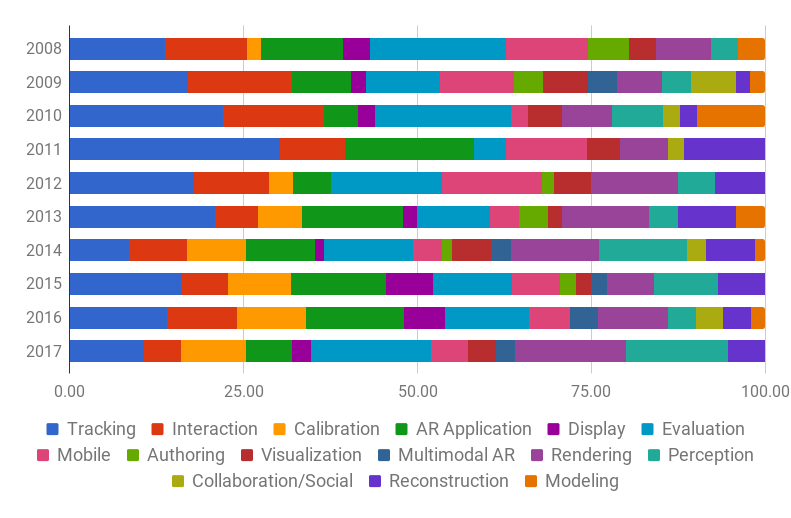
\includegraphics[width=\textwidth]{image/ismar3}
		\caption{مقابسه تمایل نویسندگان بر اساس موضوع}
		\label{fig:tiger}
	\end{subfigure}
\begin{subfigure}[b]{0.5\textwidth}
	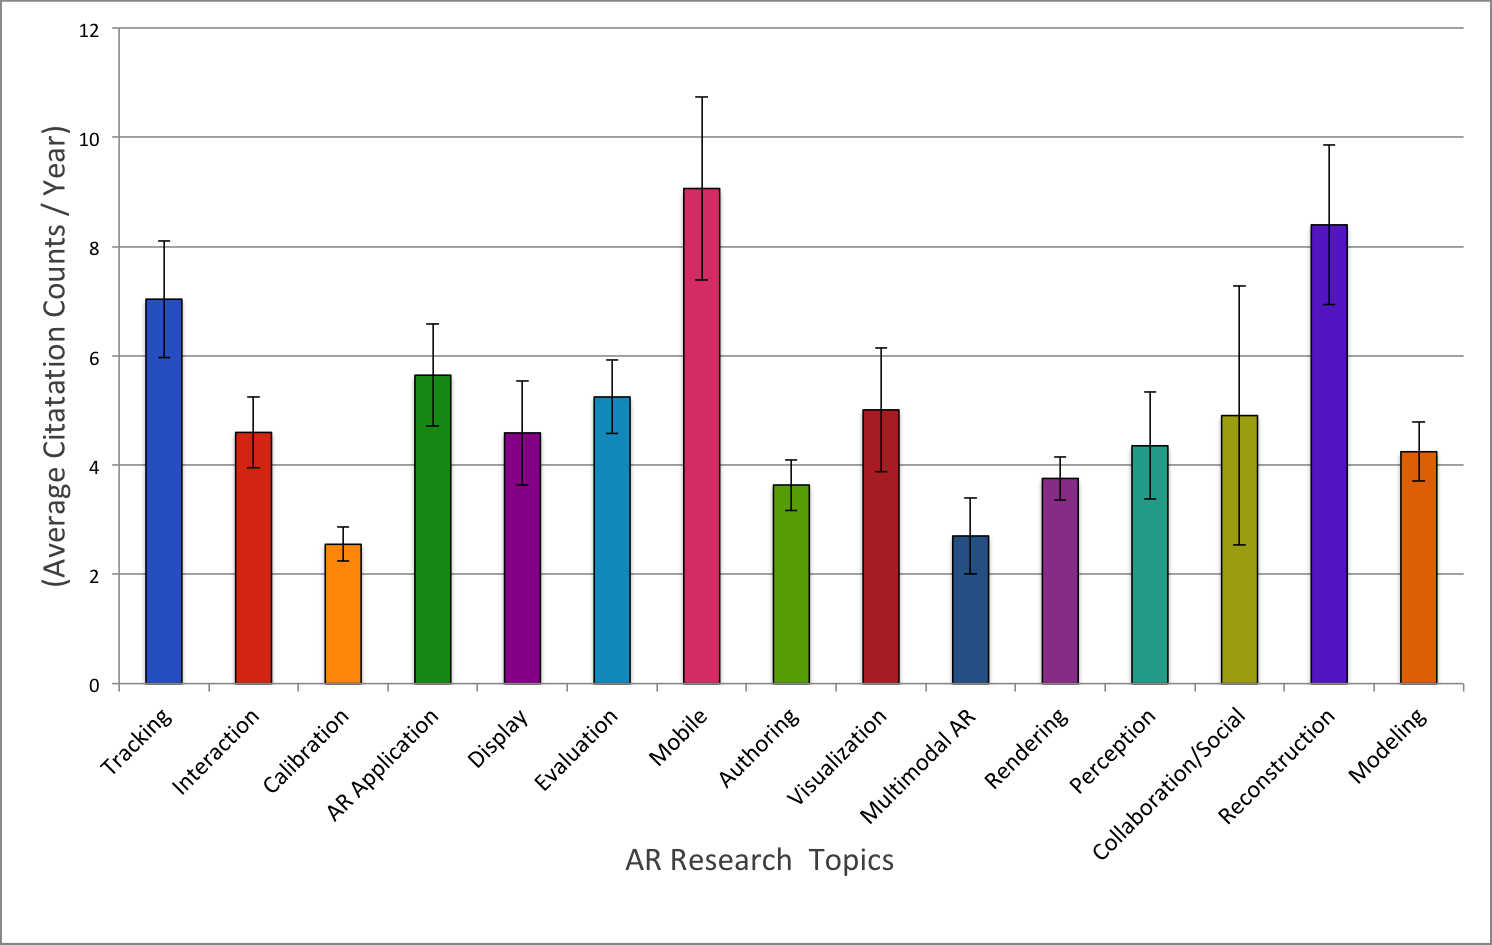
\includegraphics[width=\textwidth]{image/ismar4}
	\caption{میانگین ارجاع به مقالات در سال بر اساس موضوع}
	\label{fig:tiger}
\end{subfigure}
	\caption{بررسی 2 دهه کنفرانس ISMAR\cite{ismar}}\label{fig:ISMAR}
\end{figure}

 همان‌طور که از نتایج پیدا است یکی از حوزه‌های موردعلاقه محققین ردیابی\LTRfootnote{Tracking}، است که مقاله‌های زیادی در این حوزه منتشر می‌شود و همچنین ارجاعات به این مقالات نیز بالا می‌باشد.



\section{بیان ساختار فصل‌های بعدی}
بخش‌بندی سمینار به شکل زیر است:
\\
\textbf{
	بخش دوم:} در این بخش درخت موضوعی را به نمایش می‌گزاریم، ادبیات موضوع را مطرح کرده، کلیه اطلاعات لازم در واقعیت افزوده را شرح داده و به بیان حوزه‌های مختلف در آن می‌پردازیم و به‌اختصار آن‌ها را شرح می‌دهیم.
\\
\textbf{
	بخش سوم: } در این بخش به معرفی رندرینگ در واقعیت افزوده می‌پردازیم و اجزای آن را شرح می‌دهیم و سپس تمرکز خودمان را بر روی ردیابی (Tracking) می‌گزاریم و روش‌های مختلف درون آن را شرح می‌دهیم و کارهای گذشته را ذکر می‌کنیم.
\\
\textbf{
	فصل چهارم:} در این فصل روش‌های مختلف را باهم مقایسه کرده و مسئله‌ای را مطرح کرده و به چالش‌های آن می‌پردازیم.
\\
\textbf{
	فصل پنجم:} در این فصل به نتیجه‌گیری کلی می‌پردازیم.

\cchapter{ادبیات تحقیق}
\section{معرفی}
\subsection{انواع رابط کاربری}
\noindent
محقق \lr{Ron Azuma} بیان می‌کند که واقعیت افزوده باید شامل ۳ ویژگی باشد\cite{Azuma}:
\\
۱- باید توانایی ترکیب دنیای واقعی و مجازی را دارا باشد.
\\
۲- باید با دنیای واقعی در ارتباط باشد.
\\
۳- باید به‌صورت ۳ بعدی قابل استناد باشد.
\\
مثال شبکه خبری \lr{CNN} هر سه این شرایط را دارا می‌باشد. تصویر مجازی خبرنگار \lr{Jessica Yellin} به‌صورت زنده بر روی صحنه ظاهر شد و همچنین توانایی برقراری ارتباط و صحبت با خبرنگار \lr{Wolf Blitzer} در همان زمان بود و تصویر مجازی به‌صورت سه بعدی قابل‌نمایش بود.
\\
در یک سیستم واقعیت افزوده هر سه شرط باید رعایت شود و همچنین باید شامل یک سیستم کامپیوتری که قادر است تصاویر مجازی تولید کند و به دنیای واقعی اضافه کند باشد، همچنین باید یک سیستم ردیابی \LTRfootnote{Tracking} را دارا باشد تا بتواند نقطه مناسب برای ظاهر شدن تصویر مجازی را شناسایی بکند و تصویر مجازی را بر روی آن به نمایش درآورد. در قسمت بعدی این تحقیق مفصل به بیان سیستم ردیابی می‌پردازیم.
\\
باید توجه شود که در تعریف \lr{Azuma} هیچ محدودیتی آورده نشده در مورد نوع تکنولوژی که برای ظاهر کردن تصاویر در دنیای واقعی از آن استفاده می‌کنیم، همچنین در سیستم لزومی به‌ظاهر شدن تصویر نمی‌باشد و می‌تواند به پخش موسیقی و یا پخش فیلم بپردازد.
\\
اگر با یک دید جامع نگاه بکنیم، واقعیت افزوده آخرین تلاش توسط محققین و مهندسین برای حذف رابط کاربری در کامپیوترها و افزایش تعامل کاربر با دنیای واقعی است.\lr{Rekimoto}  تفاوت بین رابط‌های میز کار سنتی \LTRfootnote{traditional desktop computer interfaces} با تلاش‌هایی که در جهت حذف رابط کاربری انجام‌شده است را متمایز ساخت\cite{Rekimoto}. همان‌طور که در شکل \ref{fig:Rekimoto} قابل‌مشاهده است، \lr{Rekimoto} به معرفی انواع رابط‌های کاربری پرداخت و ۴ مدل را معرفی نمود.
\\
\begin{figure}[tb]
	\centering
	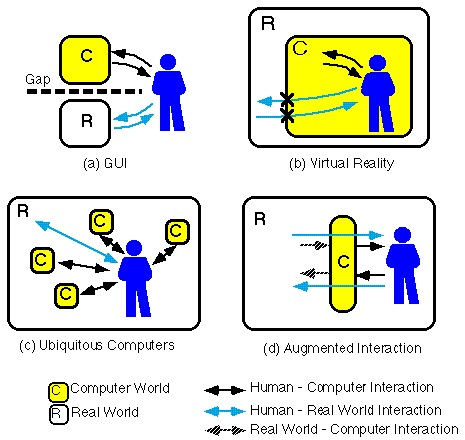
\includegraphics[width=1\linewidth]{image/style}
	\caption {انواع رابط‌های کاربری\cite{Rekimoto}}
	\label{fig:Rekimoto}
\end{figure}
\textbf{1- مدل رابط گرافیکی کاربر \lr{(GUI)}:\LTRfootnote{graphical user interface}}در این مدل کاربر با استفاده از اشکال گرافیکی که توسط کامپیوتر در اختیارش قرار می‌گیرد ارتباط برقرار می‌کند مانند آیکون‌ها، محیط ویندوز، منوها و ...
\\
\textbf{
	۲- مدل واقعیت مجازی:\LTRfootnote{Virtual Reality} }در این مدل کاربر با استفاده از کلاهی که بر روی سر و چشمانش قرار می‌گیرد وارد دنیای مجازی شده و درون این دنیا قرار می‌گیرد و با استفاده از دستکش‌ها و یا دسته‌های مخصوص شروع به تعامل با دنیای مجازی می‌کند و به‌اصطلاح درون این دنیا غواصی\LTRfootnote{immersive} می‌کند و از دنیای واقعی جدا می‌شود.
\\
\textbf{۳ -مدل پردازش همه‌جا حاضر:\LTRfootnote{Ubiquitous Computing} }در این مدل سنسورها و پردازشگرها در دنیای واقعی جاسازی‌شده‌اند.
\\
\textbf{
	۴- واقعیت افزوده:\LTRfootnote{Augmented Reality}} مشکل مدل دوم (واقعیت مجازی) این است که کاربر از دنیای واقعی جداشده و توانایی ارتباط با آن را ندارد ولی در این مدل کاربر علاوه بر توانایی تعامل با دنیای مجازی، قادر است با دنیای واقعی نیز تعامل بکند و این دو نه‌تنها مشکلی برای هم ایجاد نمی‌کنند، بلکه مکمل و کمک‌کننده به یکدیگر هستند.
\\
همان‌طور که در تعاریف بالا می‌توانیم ببینم، رابطه نزدیکی بین واقعیت مجازی و واقعیت افزوده وجود دارد، همچنین هر دو آن‌ها دارای صفحه‌نمایشی که بر روی سر نصب‌شده\LTRfootnote{head mounted displays}، سیستم ردیابی و دستگاه‌های ورودی دستی\LTRfootnote{handheld input devices} می‌باشند، بااین‌حال بین این دو تفاوت‌های مهمی وجود دارد.
\\
هدف اصلی از واقعیت مجازی، استفاده از تکنولوژی برای جایگزینی آن با دنیای واقعی است و در مقابل آن در واقعیت افزوده، تکنولوژی سعی بر آن دارد  با استفاده از محتوای دیجیتال\LTRfootnote{digital content} بدون آنکه به کاربر حس غوطه‌ور شدگی دست بدهد به دنیای واقعی بیفزاید. در واقعیت مجازی دستگاه نمایشگر باید کاملاً جامع باشد و میدان گسترده‌ای از دید را پوشش بدهد و گرافیک‌های ۳ بعدی تا حد امکان واقعی به نظر بیایند. ازآنجاکه کاربر به مدت زیادی قادر به دیدن دنیای واقعی نمی‌باشد، در واقعیت مجازی سیستم ردیابی نیاز به دقیق بودن به نسبت دنیای واقعی را ندارد و این حساسیت در آن کمتر می‌باشد.
\\
در مقابل، در  واقعیت افزوده، سیستم نمایش می‌تواند به‌صورت غیر غوطه‌ور کننده، با گستردگی دید کم و با استفاده از گرافیک‌های کوچک باشد. ولی در اینجا، سیستم ردیابی باید بسیار دقیق باشد و توانایی داشته باشد تا محتوای مجازی را دقیقاً بر روی دنیای واقعی قرار بدهد. برای کاربران واقعیت افزوده بسیار ساده است تا متوجه چندین میلی‌متر تفاوت قرار گرفتن محتوای مجازی با دنیای واقعی بشوند.
\\
\subsection{واقعیت ترکیبی}
برای توضیح بیشتر برای واقعیت افزوده می‌توانیم به نتیجه تحقیق Milgram و Kishino نگاهی بیندازیم\cite{Milgram}. آنها مفهومی با نام واقعیت ترکیبی\LTRfootnote{Mixed Reality} را معرفی نمودند که این مفهوم دو مفهوم واقعیت و مجازی را با یکدیگر ترکیب می‌کند و همچنین طبقه‌بندی‌هایی را بر اساس میزان ترکیب مجازی و واقعیت بیان می‌کند. در سمت راست محیط مجازی\LTRfootnote{Virtual Environment} را می‌بینیم، جایی که دید کاربر از جهان توسط کامپیوترهایی که تصاویر مجازی تولید می‌کنند کاملاً جایگزین شده است. در سمت مخالف، یعنی در سمت چپ ما شاهد محیط واقعی\LTRfootnote{Real Environment} هستیم که در آن کاربر هیچ‌گونه دید و درکی از عناصر مجازی ندارد و کاملاً درون دنیای واقعی قرارگرفته است. هر چه از محیط واقعی به سمت محیط مجازی حرکت کنیم، میزان عناصر مجازی در دید کاربر افزایش میابد و این محیط مابین، به دو دسته دیگر تقسیم می‌شوند. دسته واقعیت افزوده که در آن میزان واقعیت در دید کاربر خیلی بیشتر از مجازی است و دسته مجازی افزوده‌شده\LTRfootnote{Augmented Virtuality} که درون آن، بیشتر دید کاربر را عناصر مجازی تشکیل داده است و قسمت کمی را عناصر واقعی تشکیل می‌دهند.
\\
با استفاده از شکل \ref{fig:Mixed}، به این نتیجه می‌رسیم که واقعیت افزوده خود به‌تنهایی به‌عنوان دسته مجزا شناخته نمی‌شود بلکه بخشی از هر دو را تشکیل می‌دهد.

\begin{figure}[!ht]
	\centering
	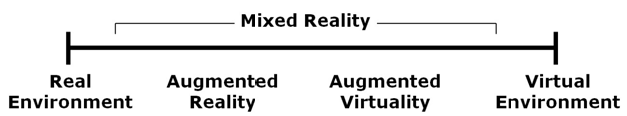
\includegraphics[width=1\linewidth]{image/mixedreality}
	\caption {شکل معرفی شده برای Reality Mixed توسط Milgram\cite{Milgram}}
	\label{fig:Mixed}
\end{figure}

\section{انواع دستگاه‌های واقعیت افزوده}

دستگاه‌های نمایشگری که با استفاده از آن‌ها تکنولوژی واقعیت افزوده را به نمایش درمی‌آوریم به سه دسته کلی تقسیم می‌شوند\cite{Julie}:
\\
\subsection{
	۱- نمایشگرهایی که بر روی سر نصب می‌شوند\protect\LTRfootnote{head mounted displays
		(HMD)} }این نوع از نمایشگرها بر روی سر قرار می‌گیرند مانند کلاه ایمنی و یا مانند عینک، در جلوی چشمان قرار داده می‌شوند و  قادر هستند هر دو تصویر از دنیای مجازی و واقعی را بر روی‌هم قرار داده و به کاربر نشان بدهند شکل. این دستگاه‌ها به دو صورت کار می‌کنند.
\begin{itemize}
	\item \textbf{1- دیدن از طریق ویدیو\LTRfootnote{Video-see-through}:} در این مدل، نیاز داریم تا کاربر، ۲ دوربین را بر روی سرخود قرار دهد و با استفاده از پردازش‌های تصاویر این دو دوربین، تصاویر ۳ بعدی از محیط را  به‌صورت زنده دریافت کنیم و همزمان با استفاده از یک کامپیوتر، تصاویر ۳ بعدی مجازی را طراحی بکنیم و با تصاویر دریافتی از دوربین‌ها، ادغام بکنیم، در این روش به دو مشکل برخورد می‌کنیم، مشکل اول کیفیت تصاویر است که وابسته به‌وضوح \LTRfootnote{resolution} دوربین‌ها و پردازشگرهای تصاویر است و همچنین وابسته به کیفیت تصویر تولیدشده توسط کامپیوتر است و مشکل بعدی این است که باید سرعت کارها در این نوع بالا باشد تا تأخیر \LTRfootnote{latency}دریافت تصاویر و پردازش و سپس نمایش را به حداقل برسانیم.
	\item \textbf{
		2- دیدن از طریق نور:\LTRfootnote{optical-see-through} }در این مدل کاربر با استفاده از لنزها، قادر است دنیای واقعی را ببیند، و با استفاده از دستگاه‌های خاص و تابش نور به لنزها، تصاویر ۳ بعدی را برای کاربر طراحی می‌کنیم. در اینجا کیفیت تصاویر دریافتی به نسبت روش قبل بالاتر است زیرا برای دیدن دنیای واقعی نیازی به‌وضوح نمایشگر نداریم ولی برای ایجاد کردن تصاویر ۳ بعدی در این روش مشکل است. همچنین به دلیل اینکه تصاویر محیط واقعی را بدون واسطه دریافت می‌کنیم، تأخیر در اینجا نیز کمتر از روش قبلی است.
\end{itemize}

\begin{figure}[tb]
	\centering
	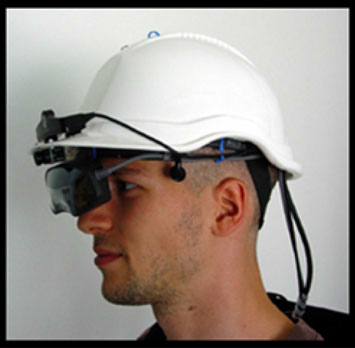
\includegraphics[width=0.6\linewidth]{image/hmd}
	\caption {نمونه‌ای از نمایشگرهای نصب‌شده بر روی سر\cite{Julie}}
	\label{fig:hmd}
\end{figure}

\subsection{نمایشگرهای دستی\protect\LTRfootnote{Handheld displays} :}
این نوع از نمایشگرها، با کمک گرفتن از دستگاه‌های محاسباتی کوچک که دارای نمایشگر می‌باشند کار می‌کنند و برای ادغام کردن تصاویر مجازی با دنیای واقعی از روش "دیدن از طریق ویدئو" استفاده می‌کنند. به‌عنوان‌مثال برای این نوع از نمایشگرها می‌توان تلفن‌های  همراه هوشمند را مثال زد که علاوه بر دارا بودن ویژگی‌های ذکرشده، دارای سنسورهایی مانند "سیستم موقعیت یاب جهانی"\LTRfootnote{Global Positioning System (GPS)} و قطب نمای دیجیتال هستند که برای ردیابی می‌توان از آن‌ها استفاده نمود
\begin{figure}[tb]
	\centering
	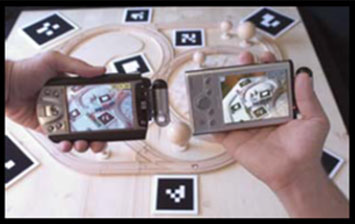
\includegraphics[width=0.7\linewidth]{image/mobile}
	\caption {نمونه‌ای از نمایشگرهای دستی\cite{Julie}}
	\label{fig:mobile}
\end{figure}
\subsection{نمایشگرهای فضایی\protect\LTRfootnote{spatial displays}}
در این نوع از نمایشگرها ما شاهد واقعیت افزوده فضایی\LTRfootnote{Spatial Augmented Reality (SAR)} هستیم که با استفاده از ویدئو پروژکتور، عناصر نوری، هولوگرام‌ها و برچسب‌های فرکانس رادیویی به‌صورت مستیم عناصر مجازی را به درون دنیای واقعی میاورند و دیگر کاربر نیازی ندارد که دستگاهی را بر روی سرخود قرار بدهد و یا اینکه دستگاهی را حمل بکند شکل\ref{fig:sar}. در نمایشگرهای فضایی، بیشتر فنّاوری بدون وابستگی به کاربر است و بدون دخالت او، عناصر مجازی را با روش اضافه کردن مستقیم\LTRfootnote{direct
	augmentation} با دنیای واقعی ادغام می‌کنیم\cite{Bimber}.
\begin{figure}[tb]
	\centering
	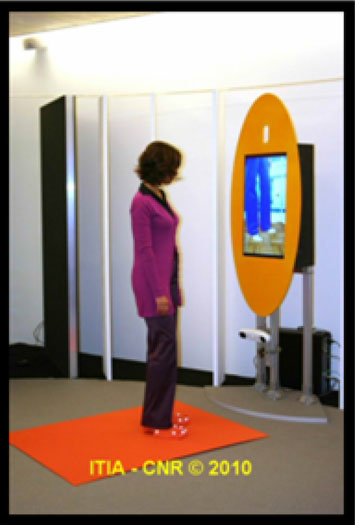
\includegraphics[width=0.6\linewidth]{image/sar}
	\caption {نمونه‌ای از نمایشگرهای فضایی\cite{Bimber}}
	\label{fig:sar}
\end{figure}
\section{ورودی و تعامل}
سیستم‌های واقعیت افزوده می‌توانند روش‌های مختلف دریافت ورودی را با یک دیگر ترکیب بکنند، مانند دریافت از صوت، دستکش‌های مخصوص، لمس کردن تصویر، پردازش تصویر و غیره. دریافت ورودی‌ها در برنامه‌های مختلف با توجه به نیاز هر برنامه متفاوت است.
سیستم‌های طراحی‌شده برای دریافت ورودی و تعامل با واقعیت افزوده را می‌توان به ۵ دسته زیر تقسیم نمود:

\subsection{مرورگرهای اطلاعات\protect\LTRfootnote{Information Browsers}: }رابطی است برای نشان دادن اطلاعات واقعیت افزوده بر روی دنیای واقعی. این نوع از دریافت اطلاعات و تعامل، نماینده‌ای از برنامه‌های واقعیت‌های افزوده است و درجایی کار می‌کنند که نمایشگر واقعیت افزوده به‌عنوان پنجره‌ای به‌سوی فضای اطلاعاتی در نظر گرفته می‌شود و وظیفه اصلی کاربر این است که این پنجره را کنترل کرده تا بتواند اطلاعات را دریافت بکند. اولین نمونه از این برنامه NaviCam شکل \ref{fig:Rekimoto} است که بر روی گوشی‌های هوشمند پیاده‌سازی شد. این نوع از برنامه‌ها نیاز به انجام تعامل‌های پایه دارد و شیوه کار آن‌ها به این صورت است که صحنه واقعیت افزوده را پردازش می‌کنند و اطلاعات برای کاربر پردازش می‌شود \cite{Rekimoto}.
\begin{figure}[tb]
	\centering
	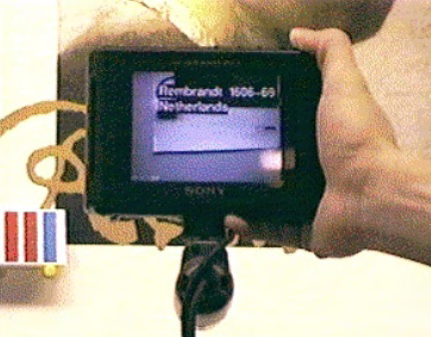
\includegraphics[width=0.6\linewidth]{image/navicam}
	\caption {نمونه‌ای از پروژه NaviCam\cite{Rekimoto}}
	\label{fig:Rekimoto}
\end{figure}
\subsection{رابط کاربر ۳ بعدی\protect\LTRfootnote{3D User Interfaces}:}
در این مدل با استفاده از تکنیک‌های تعاملی ۳ بعدی به ارتباط با محتوا در فضا می‌پردازیم. این روش یکی از راه‌های جذاب و مناسب برای تعامل است. Bowman به‌طور خلاصه این فرایند را به سه قسمت تقسیم کرده است\cite{Bowman}.
\begin{itemize}
	\item 
	\textbf{
		جهت‌یابی\protect\LTRfootnote{navigation}: }در این قسمت نیاز است که عنصر ۳ بعدی دیده شود و در اصل به سمت آن جهت‌یابی شویم، این قسمت بسیار ساده است و با حرکات بدن کاربر قابل پیاده‌سازی است. در بسیاری از دستگاه‌ها کاربر می‌تواند در سه بعد حرکت کند و در هر سه جهت نیز بچرخد.
	\item 
	\textbf{
		انتخاب\LTRfootnote{selection}:} در این قسمت نیاز است تا کاربر بتواند برای تعامل، عنصر مجازی را انتخاب بکند، برای این قسمت می‌توان از دستگاه‌های مختلف مانند سنسورها، جوی استیک\LTRfootnote{joysticks} و... استفاده کرد.
	\item 
	\textbf{
		دست‌کاری\LTRfootnote{manipulation}:} این قسمت گام آخر است و کاربر می‌تواند تعامل خود را با عناصر مجازی به‌راحتی انجام دهد.
\end{itemize}
\begin{figure}[tb]
	\centering
	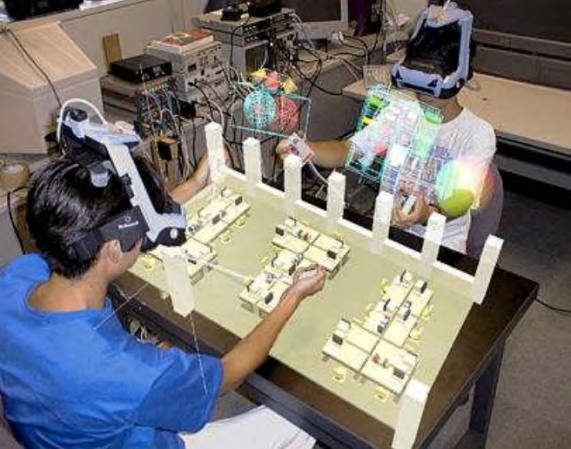
\includegraphics[width=0.6\linewidth]{image/3d}
	\caption {استفاده از رابط کاربر ۳ بعدی \cite{Bowman}}
	\label{fig:Bowman}
\end{figure}
\subsection{رابط کاربر قابل‌ لمس\protect\LTRfootnote{Tangible User Interfaces} :}
در این نوع از رابط‌ها، برای ارتباط با عناصر مجازی از عناصر دنیای واقعی استفاده می‌کنیم. این اجسام مانند پلی بین دنیای واقعی و دنیای مجازی می‌باشند و تعامل را برقرار می‌سازند. این روش یکی از روش‌های نوین برای تعامل با دنیای مجازی است، اما مشکلات خود را نیز دارا است، به‌عنوان‌مثال، وقتی‌که قصد داریم یک عنصر مجازی را بر روی عنصر فیزیکی به وجود بیاوریم، این عنصر مجازی یا باید با استفاده از پرتو تابیده شود، و یا بر روی نمایشگر کاربر ظاهر شود، در این رابط، ممکن است فاصله‌ای بین جسم مجازی و فیزیکی به وجود بیاید که ناخوشایند است\cite{Kato}.
\begin{figure}[tb]
	\centering
	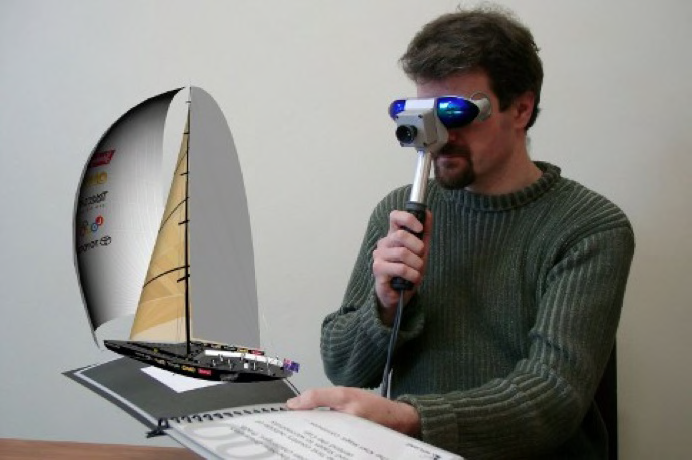
\includegraphics[width=0.6\linewidth]{image/tar}
	\caption {استفاده از رابط کاربر قابل لمس \cite{Kato}}
	\label{fig:Bowman}
\end{figure}
\subsection{رابط کاربر طبیعی \protect\LTRfootnote{Natural User Interfaces} :}
در این مدل از اجزای طبیعی بدن مانند دست‌ها استفاده می‌کنیم، در این حالت اجزای بدن می‌توانند ردیابی شوند و تشخیص داده شوند با استفاده از سنسورهای مختلفی که کاربر می‌تواند پوشیده باشد. سنسورهای مختلفی در اندازه‌ها و شکل‌های مختلفی برای این کار ساخته‌شده‌اند.
با پیشرفت کامپیوترها، سیستم‌های واقعیت افزوده توانستند حرکت و ژست بدن کاربر را بدون نیاز به سنسورها تشخیص بدهند. به‌طور مثال Lee توانست سیستمی را طراحی کند که توانایی شناسایی دست و حرکت‌های آن را داشته باشد\cite{Lee}.
\begin{figure}[!ht]
	\centering
	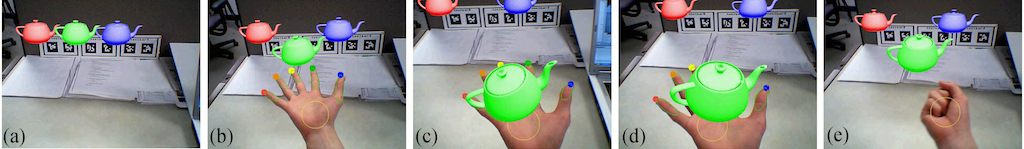
\includegraphics[width=1\linewidth]{image/handyar}
	\caption {استفاده از رابط کاربر طبیعی \cite{Lee}}
	\label{fig:Bowman}
\end{figure}

\subsection{رابط چند منظوره\protect\LTRfootnote{Multimodal Interfaces} :}
برای تعامل قوی‌تر در برنامه‌های واقعیت افزوده، محققین سعی کردند تا مدل‌های مختلفی از ورودی‌ها را با یکدیگر ترکیب کنند، در این میان ترکیب گفتار\LTRfootnote{speech} و تشخیص ژست\LTRfootnote{gesture recognition}، یکی از گسترده‌ترین و فعال‌ترین بخش‌ها بوده است.
\\
Lee در این رابطه تحقیقات زیادی انجام داد و یک سیستم چندمنظوره را طراحی کرد که در آن با استفاده از یک دوربین به  ردیابی ژست دست می‌پرداخت و همچنین با دریافت گفتار و ترکیب این دو، دستورات را شناسایی می‌کرد و به تعامل با کامپیوتر می‌پرداخت.
او توانست دقت را در این روش شناسایی کند و بیان کرد که با این ترکیب در سیستم واقعیت افزوده ۲۵ درصد سریع‌تر به نسبت تشخیص ژست به‌تنهایی، می‌توان به تعامل پرداخت\cite{Lee2}.
\begin{figure}[!ht]
	\centering
	\begin{subfigure}[b]{0.5\textwidth}
		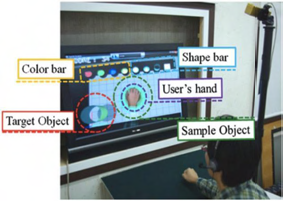
\includegraphics[width=\textwidth]{image/lee2}
		
		
	\end{subfigure}
	~ %add desired spacing between images, e. g. ~, \quad, \qquad, \hfill etc. 
	%(or a blank line to force the subfigure onto a new line)
	\begin{subfigure}[b]{0.4\textwidth}
		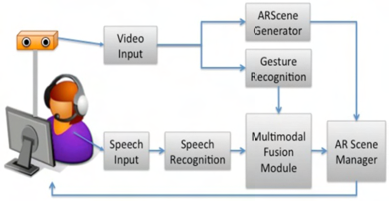
\includegraphics[width=\textwidth]{image/lee1}
		
	\end{subfigure}
	\caption{رابط چند منظوره\cite{Lee2}}\label{fig:lee2}
\end{figure}

\section{نمایش}
در واقعیت افزوده، اشیاء مجازی و دنیای واقعی باید با یکدیگر ترکیب شوند و به صورت همزمان نمایش داده
شوند. برای رسیدن به این هدف قبل از به نمایش درآمدن واقعیت افزوده چندین فرایند باید انجام شوند که
عبارتند از: کالیبره کردن دوربین\LTRfootnote{calibration}، ثبت\LTRfootnote{registration}، ردیابی و ساخت\LTRfootnote{construction}.
\\
کالیبره کردن دوربین رویه‌ای است که در آن پارامترهای دوربین مجازی با دوربین واقعی منطبق می‌شود شکل \ref{fig:Billinghurst}. 

\begin{figure}
	\centering
	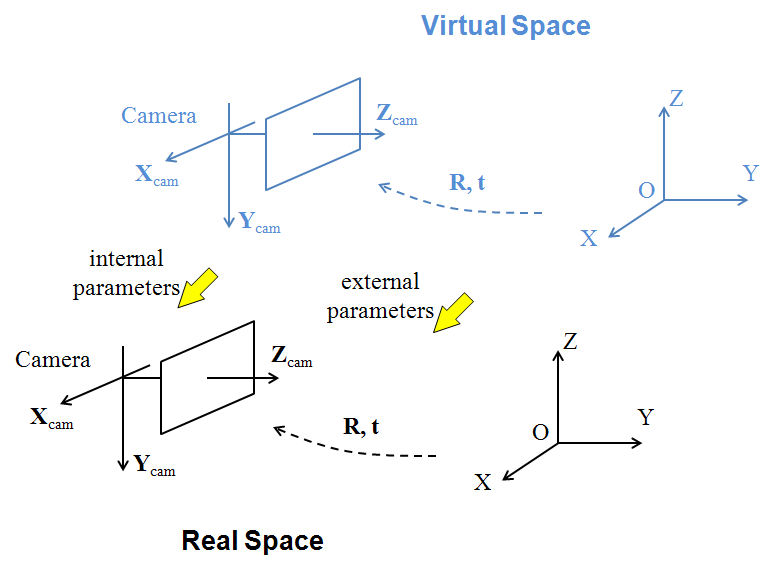
\includegraphics[width=1\linewidth]{image/realspace}
	\caption {منطبق کردن پارامترهای داخلی و خارجی \cite{Billinghurst}}
	\label{fig:Billinghurst}
\end{figure}

این امر برای نمایش صحیح اشیاء مجازی منطبق بادید کاربر، نیاز است. دوربین‌ها دارای دو نوع از پارامترها هستند، پارامترهای داخلی و پارامترهای خارجی. 

\begin{itemize}
	\item \textbf{پارامترهای داخلی، }
 پارامترهایی هستند که ساختار سه بعدی محیط را به تصویر دو بعدی تبدیل می‌کنند. پارامترهای داخلی با تهیه چندین تصویر توسط دوربین از الگوهای شناخته‌شده و مقایسه ویژگی‌های تصاویر به‌دست‌آمده از این الگوها با ویژگی‌های سه بعدی آنها، تعیین می‌شوند. این امر معمولاً قبل از شروع به‌کار سیستم واقعیت افزوده انجام می‌شود.
 \item \textbf{پارامترهای خارجی}
   با ردگیری دوربین و تعیین فاصله و جهت دوربین تعیین می‌شوند. هنگامی‌که صحنه ایستا است تنها تعیین پارامترهای خارجی دوربین در حالت اولیه کافی است ولی درصحنه‌هایی که تغییر می‌کنند به این دلیل که هر تغییری ممکن است درصحنه مجازی که قرار است به محیط واقعی اضافه شود، تغییر ایجاد کند، هر جسم مهمی که مکان آن تغییر می‌کند باید ردگیری شود\cite{Billinghurst}.
\end{itemize}
با استفاده از روش‌های ردگیری، مکان و جهت دوربین و اجسام موجود در هر صحنه مشخص می‌شود. برای آنکه صحنه مجازی به‌صورت صحیح به صحنه واقعی افزوده شود، هر صحنه مجازی باید با صحنه واقعی متناظر خود تطبیق داده شود، به این رویه، رویه ثبت گفته می‌شود. پس از تطبیق صحنه واقعی با صحنه مجازی، تصویر غنی‌شده ایجاد می‌شود که می‌تواند طبق کاربرد و فنّاوری به‌کاربرده شده به‌صورت دیجیتالی و یا به‌صورت فیزیکی نمایش داده شود.
\\
در این بخش ابتدا به بررسی انواع فناوری‌های نمایش مورداستفاده در واقعیت افزوده و سپس ازنظر نوع نمایش و فاصله محل قرارگیری از چشم کاربر بررسی می‌شوند.
\subsection{فناوری نمایش}
فناوری‌های نمایش واقعیت افزوده بسته به نوع ترکیب تصویر مجازی با تصویر واقعی به سه دسته تقسیم می‌شوند: ویدیوئی\LTRfootnote{Video based}، دید نوری\LTRfootnote{Optical see-through} و ایجاد تصویر بر روی یک سطح فیزیکی\LTRfootnote{Projection onto a physical surface}.
\subsubsection{ویدیوئی}
در این نوع نمایش ابتدا تصویر محیط واقعی را به‌وسیله دوربین به‌صورت دیجیتالی تبدیل می‌کنند و سپس تصویر مجازی به کمک روش‌های پردازش تصویر، به تصویر محیط واقعی اضافه می‌شود. در بیشتر موارد دوربین در پشت صفحه‌نمایش متصل می‌شود و اجازه دیدمستقیم به محیط را می‌دهد. درواقع در این مدل دنیای واقعی را از طریق صفحه‌نمایش می‌بینیم. دوربین می‌تواند در زوایای دیگر نیز قرار گیرد مثلاً رو به کاربر برای ایجاد یک آینه مجازی\cite{Billinghurst}.
با رایج شدن استفاده از دوربین‌های دیجیتال در رایانه‌ها، رایانه‌های لوحی و تلفن‌های هوشمند پیاده‌سازی واقعیت افزوده به‌سادگی امکان‌پذیر شده است. این امر سبب شده تا واقعیت افزوده ویدیوئی به عمومی‌ترین نوع واقعیت افزوده تبدیل شود. همچنین باوجود دوربین‌های دیجیتال و الگوریتم‌های پیشرفته ردگیری امکان افزایش دقت ترکیب تصویر واقعی با تصویر مجازی، در حد پیکسل فراهم‌شده است. یکی از مشکلات رایج این نوع واقعیت افزوده، عدم رعایت صحیح رابطه بین اجسام واقعی و مجازی است بدین‌صورت که قسمتی از جسم واقعی که نزدیک‌تر از محل قرارگیری جسم مجازی است در زیر جسم مجازی اضافه‌شده به تصویر قرار می‌گیرد\cite{Tian}.
\\
همان‌طور که در شکل \ref{fig:Tian}دیده می‌شود در سمت چپ شی مجازی به‌صورت نادرستی به محیط واقعی اضافه‌شده است و این مشکل در شکل سمت راست رفع شده است. این مشکل با به‌دست آوردن اطلاعات عمقی صحنه واقعی و مقایسه این اطلاعات با اطلاعات مجازی که باید به صحنه واقعی اضافه شود قابل‌حل است. جدیدترین روش به‌دست آوردن اطلاعات عمقی محیط استفاده از روش‌های تصویر پایه است \cite{Billinghurst}.
بدین‌صورت که با مقایسه دو تصویر و ترکیب آنها اطلاعات عمقی محیط به‌دست می‌آید. از دیگر روش‌های به‌دست آوردن عمق محیط استفاده از دوربین‌های پیمایش عمقی است که همراه با تصویر رنگی یک نقشه از اطلاعات عمقی محیط را نیز فراهم می‌کنند.
\begin{figure}
	\centering
	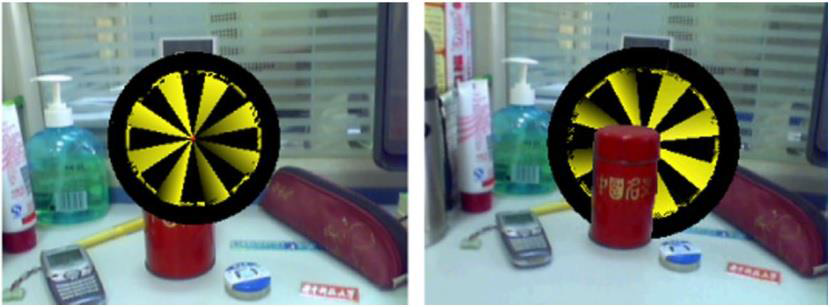
\includegraphics[width=1\linewidth]{image/wrongpic}
	\caption {اضافه شدن اشتباه در شکل سمت چپ و تصحیح آن در سمت راست \cite{Tian}}
	\label{fig:Tian}
\end{figure}


اصلی‌ترین مشکل واقعیت افزوده ویدیوئی، دید غیرمستقیم (از طریق نمایشگر) از محیط است \cite{Billinghurst}، تصویری که از طریق دوربین تهیه‌شده است دارای چندین محدودیت مانند وضوح و کیفیت تصویر، جابجایی چشم و تأخیر است. این کاستی‌ها در کاربردهایی مانند پزشکی که دیدمستقیم از محیط نیاز است بسیار مهم می‌شوند.
\\
از دیگر مشکلات این نوع نمایش، نیاز بالای قدرت پردازشی است. باوجود افزایش قدرت پردازشی در سال‌های اخیر، در مقایسه با دیگر انواع نمایش واقعیت افزوده هنوز نیاز به افزایش قدرت پردازش در این نوع واقعیت افزوده هست.

\subsubsection{نمایش دید نوری واقعیت افزوده}
این نوع از واقعیت افزوده از سیستم‌های نوری برای نمایش تصویر مجازی به همراه تصویر محیط واقعی استفاده می‌کنند. این سیستم‌ها معمولاً از جداکننده نور\LTRfootnote{beam splitters (e.g. half mirrors or combined prisms)} استفاده می‌کنند. این جداکننده تصویر واقعی را با انعکاس تصویر مجازی ترکیب کرده و نمایش می‌دهد شکل\ref{fig:optical}. بتصویر مجازی ترکیب کرده و نمایش می‌دهد شکل. بیشتر این نوع از سیستم‌ها از ملحق کننده نور، جدا از صفحه‌نمایش برای ترکیب دنیای واقعی و تصویر مجازی استفاده می‌کنند. اخیراً با پیشرفت فنّاوری صفحه‌نمایش‌هایی ساخته‌شده که شفاف هستند، استفاده از آنها در واقعیت افزوده به‌شدت روبه افزایش است. استفاده از این نوع صفحه‌نمایش‌ها باعث سادگی و کوچک شدن ساختار سیستم دید نوری واقعیت افزوده می‌شود\cite{Billinghurst}.

\begin{figure}
	\centering
	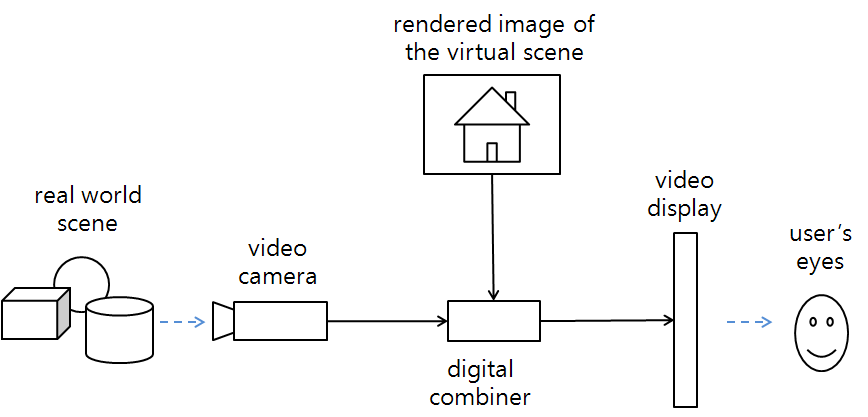
\includegraphics[width=1\linewidth]{image/opticalview}
	\caption {نمایش دید نوری \cite{Billinghurst}}
	\label{fig:optical}
\end{figure}

یکی از مهم‌ترین برتری‌هایی که این روش نسبت روش ویدیوئی دارد ایجاد دیدمستقیم از محیط واقعی است. با این امکان این نوع از واقعیت افزوده از مشکلاتی مانند تأخیر، کم بودن وضوح و غیره رنج نمی‌برد و برای کاربردهایی مناسب است که به دیدمستقیم از دنیای واقعی نیاز دارند مانند کاربردهای پزشکی و نظامی که این‌یک ویژگی بسیار مهم است.
\\
اصلی‌ترین مشکل این نوع از واقعیت افزوده دقت پایین در نگاشت دو تصویر محیط واقعی و مجازی بر روی یکدیگر است. در بیشتر پیاده‌سازی‌ها نیاز به کالیبره کردن رویه ثبت است که معمولاً دقت پایین‌تری نسبت به رویه‌های خودکار موجود در واقعیت افزوده ویدیوئی دارند. به این دلیل که پارامترهای کالیبره کردن تصاویر واقعی و مجازی به نسبت زیادی وابسته به فضای بین چشم کاربر و صحنه موردنظر است و این فضا در طول زمان تغییر می‌کند و باعث ایجاد خطا در نگاشت دو تصویر واقعی و مجازی بر یکدیگر می‌شود \cite{Billinghurst}.
\\
یکی دیگر از مشکلات واقعیت افزوده دید نوری تأخیر موقتی بین نمایش تصویر مجازی و دیده مستقیم واقعی است. باوجود سیستم ردگیری دقیق بازهم یک تأخیر موقتی بین نمایش تصویر مجازی و دید دنیای واقعی وجود دارد.
\\
در بسیاری از موارد، ایجاد رابطه صحیح عمقی بین دنیای واقعی و مجازی در واقعیت افزوده دید نوری مشکل است. با توجه به ماهیت نیمه شفاف ترکیب‌کننده تصاویر، کاربران یک دید نیمه شفاف از تصویر دنیای واقعی و مجازی دارند. به‌صورتی که، هیچ‌کدام دیگری را تماماً نمی‌پوشاند. Kiyokawa و همکاران\cite{Kiyokawa} برای رفع این مشکل یک ماسک الکترونیکی برای پوشاندن مکان‌هایی که اشیاء مجازی اضافه می‌شوند طراحی کرد. با بستن پیکسل‌هایی از صفحه‌نمایش که اشیای مجازی در آن پیکسل‌ها قرار می‌گیرند دید دنیای واقعی بسته‌شده و اشیاء مجازی واضح‌تر به نمایش درمی‌آیند.
\\
شرایط نوری محیط می‌تواند در دید واقعیت افزوده دید نوری تأثیرگذار باشد. در اکثر مواقع ترکیب‌کننده نوری دارای شفافیت ایستا است که می‌تواند باعث خطا در میزان روشنایی تصویر مجازی و دید محیط واقعی شود. در محیط‌های بیرونی اشیاء مجازی باید تیره‌تر از تصویر محیط واقعی به نمایش درآیند. برای رفع این مشکل نمایشگرهای متصل به سر به چندین کاور با میزان شفافیت متفاوت مجهز شده‌اند.
\subsubsection{نمایش مبتنی بر نورپردازی}
واقعیت افزوده مبتنی بر نورپردازی سطح یک جسم واقعی را به کمک نورپردازی با تصویر مجازی می‌پوشاند شکل\ref{fig:tajmahal}. با توجه به ترکیب ردگیری زاویه دید کاربر و سطح فیزیکی اجسام، واقعیت افزوده مبتنی بر نورپردازی دارای قابلیت اضافه کردن تعاملی را دارد\cite{Raskar}. در بیشتر مواقع برای این منظور از ویدئو پروژکتور متصل به سقف و یا دیوار برای پوشاندن سطح اجسام استفاده می‌شود. این امر سبب می‌شود که قابلیت جابجایی وجود نداشته باشد و محدود به مکانی باشد که پروژکتور می‌تواند نورپردازی کند. البته در سال‌های اخیر تلاش‌هایی برای ایجاد قابلیت جابجایی برای ویدئو پروژکتورها شده است که می‌توان به نمونه‌هایی که قابلیت قرار گرفتن در دست\cite{Mistry} و متصل شدن به سر است\cite{krum2012augmented} اشاره کرد.

\begin{figure}
	\centering
	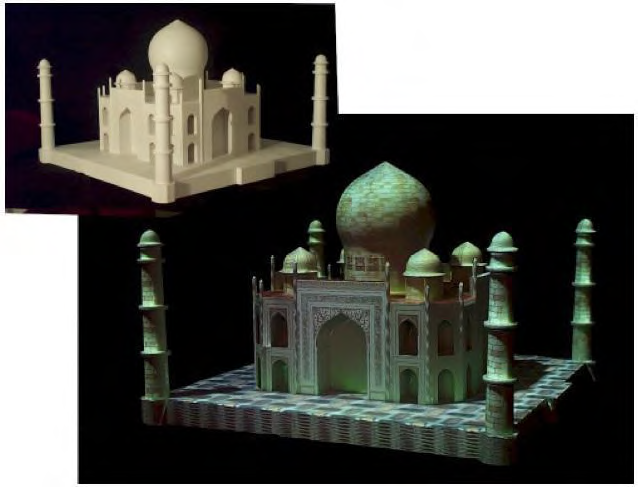
\includegraphics[width=1\linewidth]{image/tajmahal}
	\caption {نمایش دید نوری \cite{Mistry}}
	\label{fig:tajmahal}
\end{figure}

یکی از محدودیت‌های واقعیت افزوده مبتنی بر نورپردازی، نیازمند بودن به سطح یک جسم برای نمایش تصویر مجازی است که باعث می‌شود تنها اجسام نزدیک به پروژکتور مناسب باشند و در استفاده برای کاربردهای شهری محدودیت ایجاد می‌کند. همچنین این نوع از واقعیت افزوده وابستگی بیشتری به شرایط نوری محیط دارد چراکه سایه دیگر اجسام می‌تواند مشکل‌ساز باشد. همچنین ایجاد رابطه صحیح عمقی بین سطح جسم موردنظر و دیگر اجسام مشکل است.

\subsection{فاصله قرار گیری نمایشگر}
یکی دیگر از جنبه‌های نمایش واقعیت افزوده فاصله نمایشگر از چشم کاربر است که می‌توانند در دسته‌هایی مانند نمایشگر متصل به سر\LTRfootnote{Head-attached Displays}، نمایشگر دستی و یا متصل به بدن\LTRfootnote{Handheld and Body-attached Displays} و نمایشگر فاصله‌دار\LTRfootnote{Spatial Displays} قرار گیرند.

	content...

\subsubsection{نمایشگر متصل به سر}
این نوع نمایشگر تصویر مجازی را درست در جلوی چشمان کاربر نمایش می‌دهد، که در این صورت جسم دیگری مانع دیدن تصویر نمی‌شود. این نوع نمایشگرها در اندازه‌های مختلف وجود دارند که از اندازه یک کلاه تا اندازه یک عینک متفاوت است. به همان نسبت که حمل و متصل کردن آن به سر راحت‌تر می‌شود، تصویر عریض‌تر و درخشان‌تر می‌شود\cite{Billinghurst}.
\subsubsection{نمایشگر دستی و یا متصل به بدن}
نمایشگر متصل به سر دارای قابلیت‌هایی مانند قابلیت حمل بالا و فراهم کردن تصویر فراگیر است اما به دلیل پوشیدنی بودن آنها در بعضی از موارد دارای محدودیت هستند. نمایشگرهای در دست گرفتنی و یا متصل به بدن به‌عنوان نمایشگرهای شخصی و قابل‌حمل در نظر گرفته می‌شوند و در صورت نیاز قابل به اشتراک‌گذاری با دیگران هستند. آنها همچنین ازنظر اجتماعی قابل پذیرش تر از نمایشگر متصل به سر هستند.
\\
با پیشرفت فنّاوری درزمینه دستگاه‌های قابل‌حمل، قدرت پردازشی دستگاه‌های قابل‌حمل برای پردازش تصویرسازی واقعیت افزوده به میزان لازم افزایش پیداکرده است. اخیراً آزمایش‌هایی برای استفاده از سنسورهای عمقی بر روی رایانه‌های لوحی و تلفن‌های هوشمند انجام‌شده است (مانند پروژه تانگو گوگل.) \protect\LTRfootnote{https://developers.google.com/tango}

\begin{figure}
	\centering
	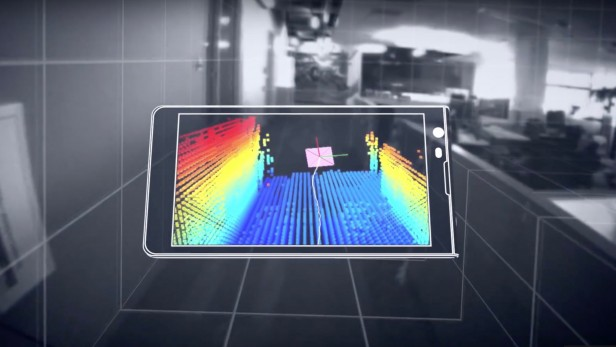
\includegraphics[width=1\linewidth]{image/tango}
	\caption {پروژه تانگو گوگل که با استفاده زا نمایشگرهای دستی کار می‌کند}
	\label{fig:tango}
\end{figure}
\subsubsection{نمایشگر فاصلهای}
این نوع از نمایشگر در مقایسه با دو نوع قبلی قابلیت حمل کمتری دارد و معمولاً در یک مکان ثابت نصب می‌شود. به این دلیل که این نوع نمایشگرها دارای اندازه بزرگی هستند. درنتیجه، برای استفاده در مکان‌های عمومی و کاربردهایی که چندین کاربر دارند مناسب هستند. از نمونه‌های این نوع نمایشگر می‌توان به نمایشگرهای رومیزی که با یک دوربین در تماس هستند اشاره کرد. از دیگر نمونه‌های آن ساخت آینه مجازی است که از یک نمایشگر بزرگ و یک دوربین رو به کاربر تشکیل‌شده است و تصویر کاربر به همراه اطلاعات مجازی اضافه‌شده در آن نمایش داده می‌شود\cite{Billinghurst}.*/



\cchapter{کارهای مرتبط}
\section{معرفی فصل}
همان‌طور که در شکل ... می‌بینیم، ما درخت موضوعی برای واقعیت افزوده را درآوردیم و در بخش دوم به بیان عناصر آن پرداختیم.
واقعیت افزوده را به همراه مثال‌های آن در بخش‌های اول و دوم بررسی کردیم، سپس انواع دستگاه‌هایی که می‌توان بر روی آن‌ها واقعیت افزوده را پیاده‌سازی کرد معرفی کردیم و مختصر روش‌های تعامل و دریافت ورودی در این سیستم را بررسی کردیم و همچنین انواع روش‌های نمایش در این سیستم را طبقه‌بندی کرده و روش کار را شرح دادیم.
\\
همان‌طور که در بخش دوم اشاره شد، محقق Azuma بیان می‌کند که واقعیت افزوده باید ۳ ویژگی داشته باشد\cite{Azuma}:
\\
۱- باید توانایی ترکیب دنیای واقعی و مجازی را دارا باشد.
\\
۲- باید با دنیای واقعی در ارتباط باشد.
\\
۳- باید به‌صورت ۳ بعدی قابل استناد باشد.
\\
برای شرط سوم، باید سیستم واقعیت افزوده ما قابلیت ثبت شدن\LTRfootnote{registration} به‌صورت ۳ بعدی را دارا باشد به معنای دیگر باید بتواند به‌صورت جزئی از دنیای واقعی به نظر بیاید. در این بخش ‌بر روی فنّاوری که این نیاز را برطرف می‌کند تمرکز می‌کنیم.
\\
\section{رندرینگ به چه معنا است؟}
در حوزه واقعیت افزوده، ۳ واژه بسیار مهم وجود دارد به نام ردیابی\LTRfootnote{Tracking}، کالیبراسیون\LTRfootnote{Calibration} و ثبت\LTRfootnote{Registration} که زیرمجموعه رندریگ\LTRfootnote{Rendering} می‌باشند و در کنار هم به این واژه معنا می‌دهند. این ۳ واژه همیشه همراه هم هستند و در یک هدف قرار دارند. برای ثبت پویا\LTRfootnote{dynamic}، نیاز به داشتن ردیابی هستیم. عناصر درون سیستم واقعیت افزوده ثبت می‌شوند و سپس در یک سیستم هماهنگ، این عناصر ثبت‌شده به دنیای واقعی پیوند\LTRfootnote{aligned} می‌شوند. در واقعیت افزوده هدف اصلی این است که اطلاعات مجازی دقیقاً به‌صورتی که از قبل برنامه‌ریزی‌شده‌اند، ثبت بشوند. کالیبراسیون به‌صورت دقیق اطلاعات حس‌گرها\LTRfootnote{sensor} را دریافت و پردازش می‌کند و مسئولیت ثبت ایستا\LTRfootnote{dynamic} با این فرایند است\cite{siltanen2012theory}.
\\
\begin{figure}
	\centering
	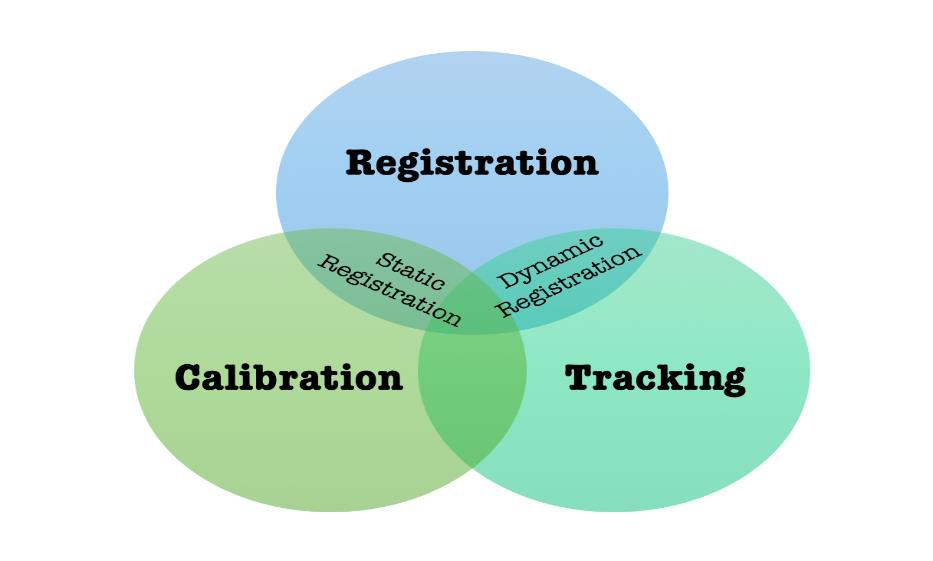
\includegraphics[width=1\linewidth]{image/rct}
	\caption {ارتباط ثبت، ردیابی و کالیبراسیون\cite{siltanen2012theory}}
	\label{fig:rct}
\end{figure}

ردیابی واژه‌ای است که برای حس کردن و محاسبه کردن مقادیر در واقعیت افزوده به‌کار می‌رود. برای تبدیل کردن موقعیت در ۳ بعد عناصر مجازی، به موقعیت‌های نسبی، نیاز به جهت‌یابی داریم. واقعیت افزوده به‌صورت بلادرنگ کار می‌کند درنتیجه برای ارسال مقدار از محیط واقعی باید به‌صورت بلادرنگ\LTRfootnote{real time} عمل کرد و همین‌طور این کار باید پیوسته در زمان صورت بگیرد. ردیابی درون سیستم‌های رایانه‌ای برای اجسام ۲ بعدی کاری رایج است اما سختی کار در اینجا ردیابی در محیط بیرون و در سه جهت مختصات برای همه‌ی نوع‌های عناصر است\cite{siltanen2012theory}.
\\
به عملیات مقایسه کردن مقادیر بین دو دستگاه، کالیبراسیون گفته می‌شود. یکی بین دستگاه مرجع\LTRfootnote{reference} و دیگری بین دستگاهی که نیاز دارد اطلاعات کالیبره شده را دریافت بکند. مختصاتی که از محیط واقعی میدانیم را به دستگاه مرجع می‌دهیم  . برخلاف ردیابی که باید به‌صورت پیوسته انجام شود، عملیات کالیبراسیون در بخش‌های مختلف زمانی و به‌صورت گسسته انجام می‌شود و برای هر دستگاه فقط یک بار این کار صورت می‌گیرد مگر اینکه دستگاه دچار مشکل بشود. کیفیت کاری دستگاه‌های واقعیت افزوده وابستگی زیادی به عملیات کالیبراسیون دارد\cite{siltanen2012theory}.
\\
به فرایند پیوند زدن مختصات عناصر مجازی با واقعی، ثبت میگوییم. به‌طور مشخص نمایشگر واقعیت افزوده باید باکیفیت بالا، عناصر مجازی را نشان دهد و یا اینکه به عناصر واقعی پیوند بزند. برای این کار نیاز داریم تا عملیات ردیابی به‌صورت کامل کار خود را انجام دهد. اگر موقعیت دوربین ثابت باشد، ما فقط با عملیات ثبت و کالیبراسیون می‌توانیم مختصات بین عناصر مجازی و واقعی را تشخیص بدهیم ولی اگر دوربین خاصیت جابه‌جایی داشته باشد، ما به عملیات ردیابی نیز، نیاز داریم\cite{siltanen2012theory}.
\\برای آوردن عناصر مجازی به دنیای واقعی، نیاز به یک لنگر\LTRfootnote{anchor} داریم که باید ژست (جهت\LTRfootnote{position} و موقعیت\LTRfootnote{orientation)}) آن مشخص باشد، این لنگر باید متعلق به دنیای واقعی باشد و می‌تواند شکل‌های مختلفی به خود بگیرد، به‌عنوان‌مثال می‌تواند یک منبع مغناطیسی باشد، یا نشانگر تصویر کاغذی\LTRfootnote{paper image marker} و یا موقعیت جغرافیایی که بر اساس سیستم موقعیت‌یاب جهانی تشخیص داده می‌شود.
\\
وابسته به نوع فنّاوری که استفاده می‌شود پروسه ثبت می‌تواند به یکی و یا هر دو فاز زیر تقسیم شود.


\textbf{فاز ثبت:}
در این فاز، ژست عنصری که در حال مشاهده است با توجه به دنیای واقعی مشخص می‌شود.

\textbf{فاز ردیابی:}
در این فاز، ژست عنصری که در حال مشاهده آن هستیم را به‌صورت نسبی اندازه‌گیری می‌کنیم.

در این بخش مطابق با اصطلاحات رایج از کلمه ردیابی برای هر دو فاز استفاده می‌کنیم و در ادامه روش‌های رایج برای ردیابی که در جهت ثبت استفاده می‌شود را بیان می‌کنیم.
\section{ردیابی مغناطیسی}
ردیابی مغناطیسی از خواص میدان‌های مغناطیسی به‌منظور محاسبه ژست یک گیرنده  که به‌عنوان یک لنگر در دنیای واقعی شناخته می‌شوند، با توجه به فرستنده استفاده می‌کند. در این مدل، فرستنده یک میدان مغناطیسی را به‌صورت متناوب تولید می‌کند که توسط یک و یا چند حسگر این اطلاعات دریافت می‌شود. با محاسبه قطب\LTRfootnote{polarization} و گرایش\LTRfootnote{orientation} میدان مغناطیسی دریافت شده، ژست دریافت‌کننده با سرعت بالایی قابل‌محاسبه است.
\\
زمانی که از این معیار در سیستم واقعیت افزوده استفاده می‌کنیم، ردیاب مغناطیسی فرستنده به‌عنوان منشأ سیستم مختصات مجازی عمل می‌کند، و با نصب کردن یک دریافت‌کننده در عنصری که سعی در دیدن آن داریم، موقعیت و جهت آن قابل‌محاسبه است\cite{caudell1992augmented}. 
\\
ردیاب‌های مغناطیسی نرخ بروز رسانی بالایی دارند و همچنین دریافت‌کننده آن‌ها کوچک و سبک هستند. ولی باید توجه داشت که قدرت میدان مغناطیسی با مکعب فاصله رابطه عکس دارد و همچنین دقت آن با توان ۴ فاصله رابطه عکس دارد. همچنین ردیابی مغناطیسی دارای معایب دیگری نیز می‌باشد مثلاً مستعد نوسان اندازه‌گیری\LTRfootnote{measurement jitter} است و نسبت به مواد مغناطیسی و میدان‌های الکتریکی در محیط واقعی حساس است.
\\
شکل\ref{fig:magnetic} نشان‌دهنده وضوح در ردیابی مغناطیسی دستگاه‌های Polhemus است که تأثیر فاصله بین دریافت‌کننده و فرستنده را نمایش می‌دهد. همان‌طور که قابل‌مشاهده است در فاصله‌های پایین این خطا بسیارکم است اما با افزایش فاصله به‌صورت نمادی خطا افزایش میابد.
\begin{figure}
	\centering
	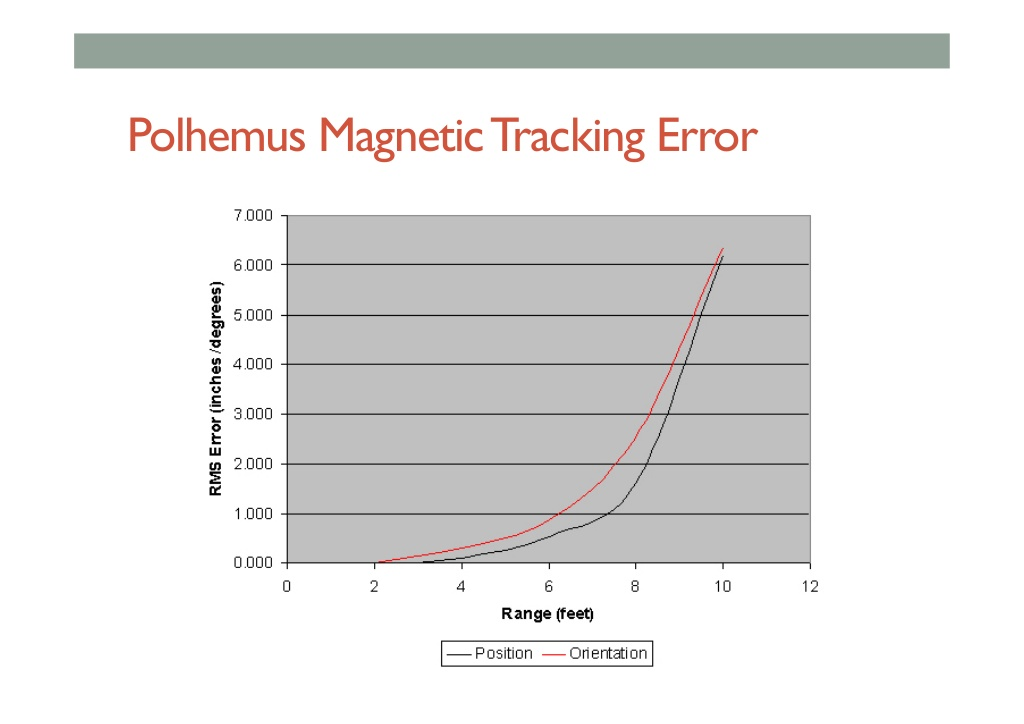
\includegraphics[width=1\linewidth]{image/magnetic}
	\caption {ارتباط فاصله با وضوح محاسبات در ردیابی مغناطیسی\protect\LTRfootnote{https://polhemus.com}}
	\label{fig:magnetic}
\end{figure}
ردیابی مغناطیسی در طیف وسیعی از سامانه‌های واقعیت افزوده استفاده‌شده است، مانند برنامه‌هایی در حوزه‌های تولید\cite{caudell1992augmented}، نگهداری\cite{feiner1993knowledge}، سلامت\cite{bajura1992merging}.
\section{ردیابی براساس دید}



%%%%%%%%%%%%%%%%%%%%%%%%%%%
	

% مراجع
\newpage
%\onehalfspacing
\bibliographystyle{ieeetr-fa}%{chicago-fa}%{plainnat-fa}%
\bibliography{thesis}


%%%%%%%%%% نمونه‌ی واژه‌نلمه تک ستونه ٪٪٪٪٪٪٪٪٪٪
\baselineskip=.6cm

\chapter*{واژه‌نامه  انگلیسی به  فارسی}\markboth{واژه‌نامه  انگلیسی به  فارسی}{واژه‌نامه  انگلیسی به  فارسی}
%\thispagestyle{fancy}
\addcontentsline{toc}{chapter}{واژه‌نامه  انگلیسی به  فارسی}
\noindent
\englishgloss{Word}{کلمه}
\englishgloss{Word 2}{کلمه ۲}
\englishgloss{Word 3}{کلمه ۳}


\chapter*{واژه‌نامه فارسی به انگلیسی}\markboth{واژه‌نامه فارسی به انگلیسی}{واژه‌نامه فارسی به انگلیسی}
\addcontentsline{toc}{chapter}{واژه‌نامه فارسی به انگلیسی}
%\thispagestyle{fancy}
\noindent
\persiangloss{کلمه ۱}{word 1}
\persiangloss{کلمه ۲}{word 2}
\persiangloss{کلمه ۳}{word 3}

\baselineskip=1cm
%%%%%%%%%%%%%%%%%%%%%%%%%


% چکیده به انگلیسی
\en-abstract
{
	This is Abstract in English.
}

% کلمات کلیدی انگلیسی 
\latinkeywords
{
	Word1, Word2, Word3
}

\latinAbstractPage % ساخت صفحه چکیده به انگلیسی
\latinFirstPage % ساخت صفحه آخر

	
\end{document}